\documentclass[a4paper,20pt]{article}
\usepackage{amsmath}
%\usepackage[a4paper, total={15cm, 20cm}]{geometry}
\usepackage{graphicx}
\usepackage{hyperref}
\usepackage{indentfirst}
\hypersetup{colorlinks=true, linkcolor=blue}

%% Documents settings
\title{Projet Optimisation}
\author{Vasavan \& Wesley}

\begin{document}
%% Generate the title
\maketitle
\newpage
\protect\hypertarget{table}{}
\renewcommand{\contentsname}{Sommaire}
\tableofcontents
\newpage
\newpage

\section{Objectif}
La mission d'un lanceur spatial est d'amener un satellite en orbite. Le
 probl\`eme est divis\'e en deux parties l'impl\'ementation de l'algorithme SQP
 (Sequential Quadratic Programming) et l'impl\'ementation d'un simulateur, le
 tout en \textit{Matlab}.
\newpage

\section{Algorithme et logiciel}
\subsection{Optimisateur SQP}
L'algorithme SQP permet de r\'esoudre des probl\`emes non lin\'eaires sous
 contraintes.

\begin{figure}[h!]
\centering
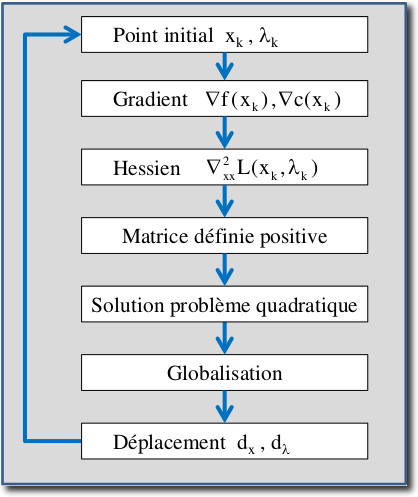
\includegraphics[width=6cm]{capture.png}
\caption{Organigramme}
\label{fig:1}
\end{figure}

\subsection{Calcul du gradient}
Le calcul du gradient de la fonction co\^ut f et de
la fonction contrainte est fait par la méthode des diff\'erences finies.

\subsection{Calcul du hessien}
Le calcul du hessien est fait par une m\'ethode de Quasi-Newton. Les it\'erations
sur le hessien sont faites soit par la méthode BFGS ou soit par la méthode SR1.

\subsection{Probl\`eme quadratique}
Cette partie r\'esolve le probl\'eme quadratique en prenant en argument la matrice hesienne d\'efinie positive,
les gradients des fontcions co\^ut f et de la fonction contrainte.

\subsection{Globalisation}
Cette partie est compos\'e de plusieurs \'etapes. On v\'erifie tout d'abord que la fonction de m\'erite est d\'ecroissante,
si elle ne l'est pas on r\'einitialise le Hessien, puis on recherche une direction de d\'escente en augmentant $\rho$.

\section{Test de validation de l'optimiseur SQP}
Plusieurs cas test sont effectu\'es pour valider l'optimiseur SQP. Les cas test sont : MHW4D et Ariane.


\subsection {Cas test: MHW4D}.

Tableau des valeurs initiales

Tableau des valeurs finales

\subsection{Cas test: Ariane}

Tableau des valeurs initiales

Tableau des valeurs finales

\section{Lanceur spatial}
La simulation du lanceur spatial est divis\'e en deux parties majeures : le probl\'eme d'\'etagement et le probl\'eme de trajectoire.

\subsection{Probl\`eme d'\'etagement}

Le probl\`eme d'\'etagement est un probl\`eme d'optimisation des masses d'\'ergols de la fus\'ee.
Il est r\'esolu par l'optimiseur SQP.


\subsection{Probl\`eme de trajectoire}

La trajectoire du lanceur est d\'ecoup\'e en trois s\'equences correspondant au fonctionnement successif des trois \'etages propulsifs.
La simulation de la trajectoire est mod\'elis\'ee par des \'equations de Mouvements que l'on r\'esout par int\'egration num\'erique, en utilisant la fonction ODE45 de Matlab.

\subsection{Optimisation des angles}

 Pour avoir un trajectoire optimis\'e, on r\'esout finalement le probl\'eme suivant sur les angles, en utilisant l'algorithme SQP :

\section{Simulation du lanceur}
\subsection{Visualisation}

\section{Probl\`emes et limites rencontr\'es}


\end{document}
